% Appendix B: figures not (yet) in the main text, for review. Captions from the archived outline.
\section{Additional figures}\label{app:figures}
\begin{notes}
\item Sensor paths with two and one shot (companions of Fig.~\ref{fig:paths}), specimen drawing, setup photo.
\item Removed from the paper 25 Nov (files kept in figures/): the 13 gradient/random pairs (F8\_pairs), and the fixed-budget figures F8b (matched budget), F8c (detection curves), F8d (fixed rate); their content is in Figs.~\ref{fig:funnel} and \ref{fig:slopes}.
\end{notes}


\begin{figure}[ht]\centering
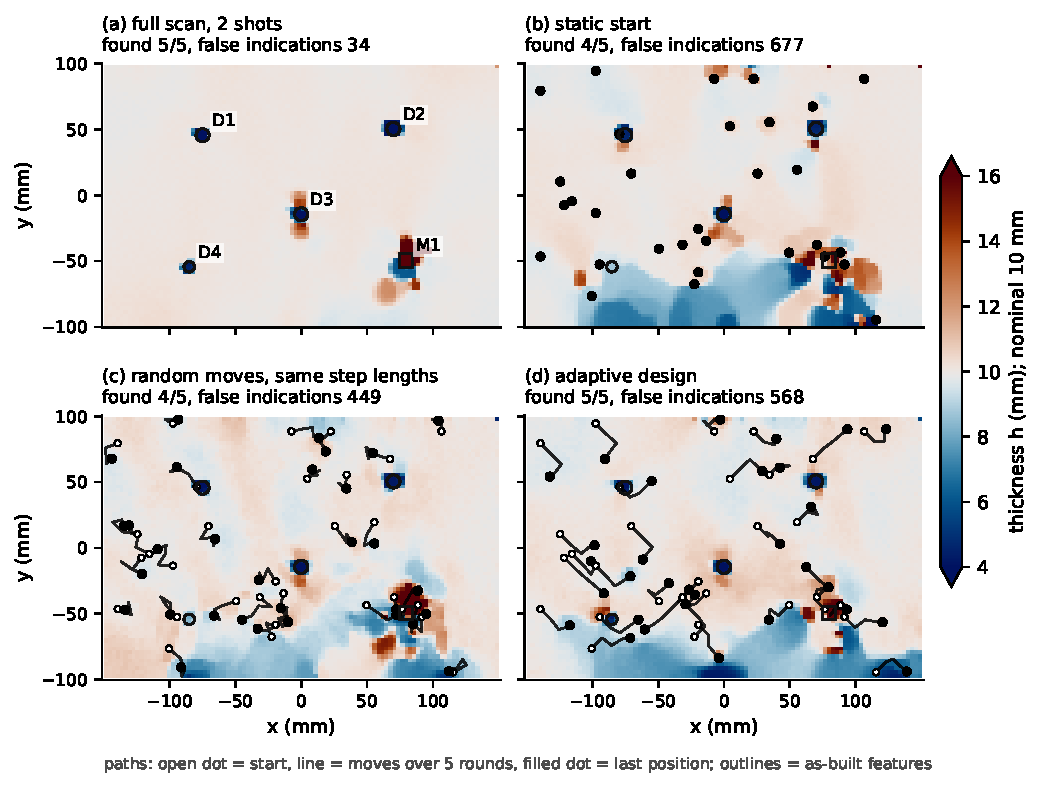
\includegraphics[width=0.9\linewidth]{F9_paths_a2_x48c.pdf}
\caption{\textbf{2 shots} (best adaptive run, x48c start): all five features found, but a thin band along the lower edge (568 false indications).}\label{fig:paths-2}
\end{figure}

\begin{figure}[ht]\centering
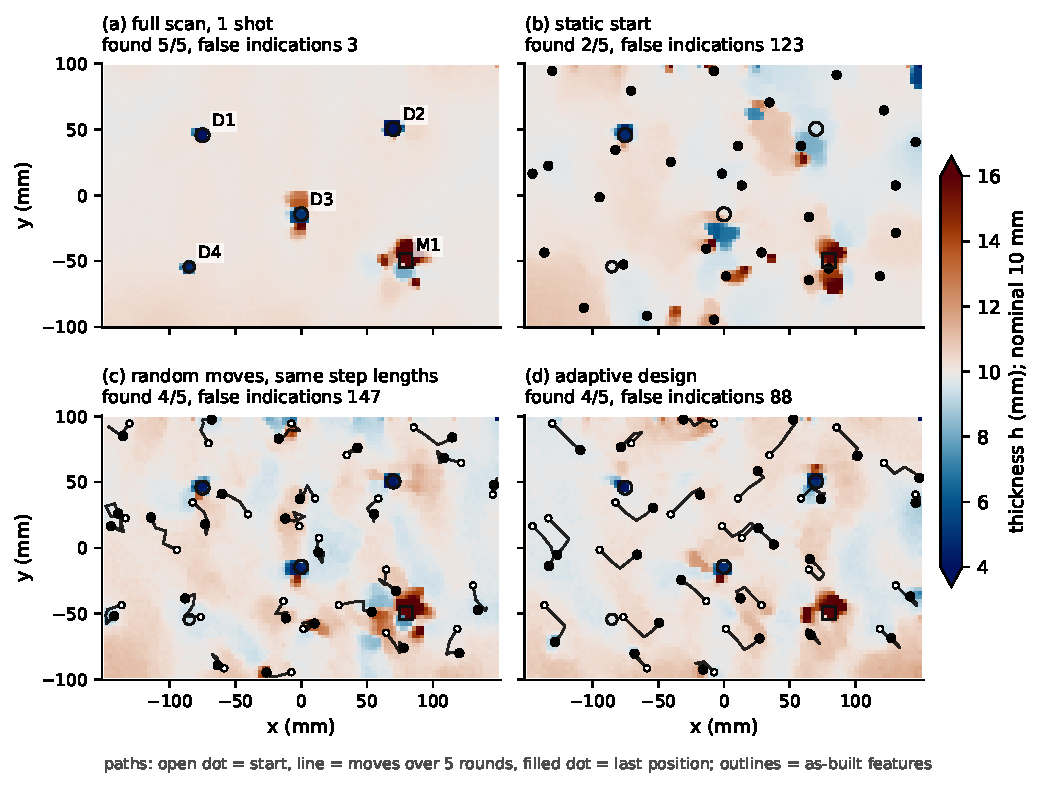
\includegraphics[width=0.9\linewidth]{F9_paths_a1_j30b.pdf}
\caption{\textbf{1 shot} (best adaptive run, j30b start): 4 of 5 found with 88 false indications, against 2 of 5 for the static start.}\label{fig:paths-1}
\end{figure}




\begin{figure}[ht]\centering
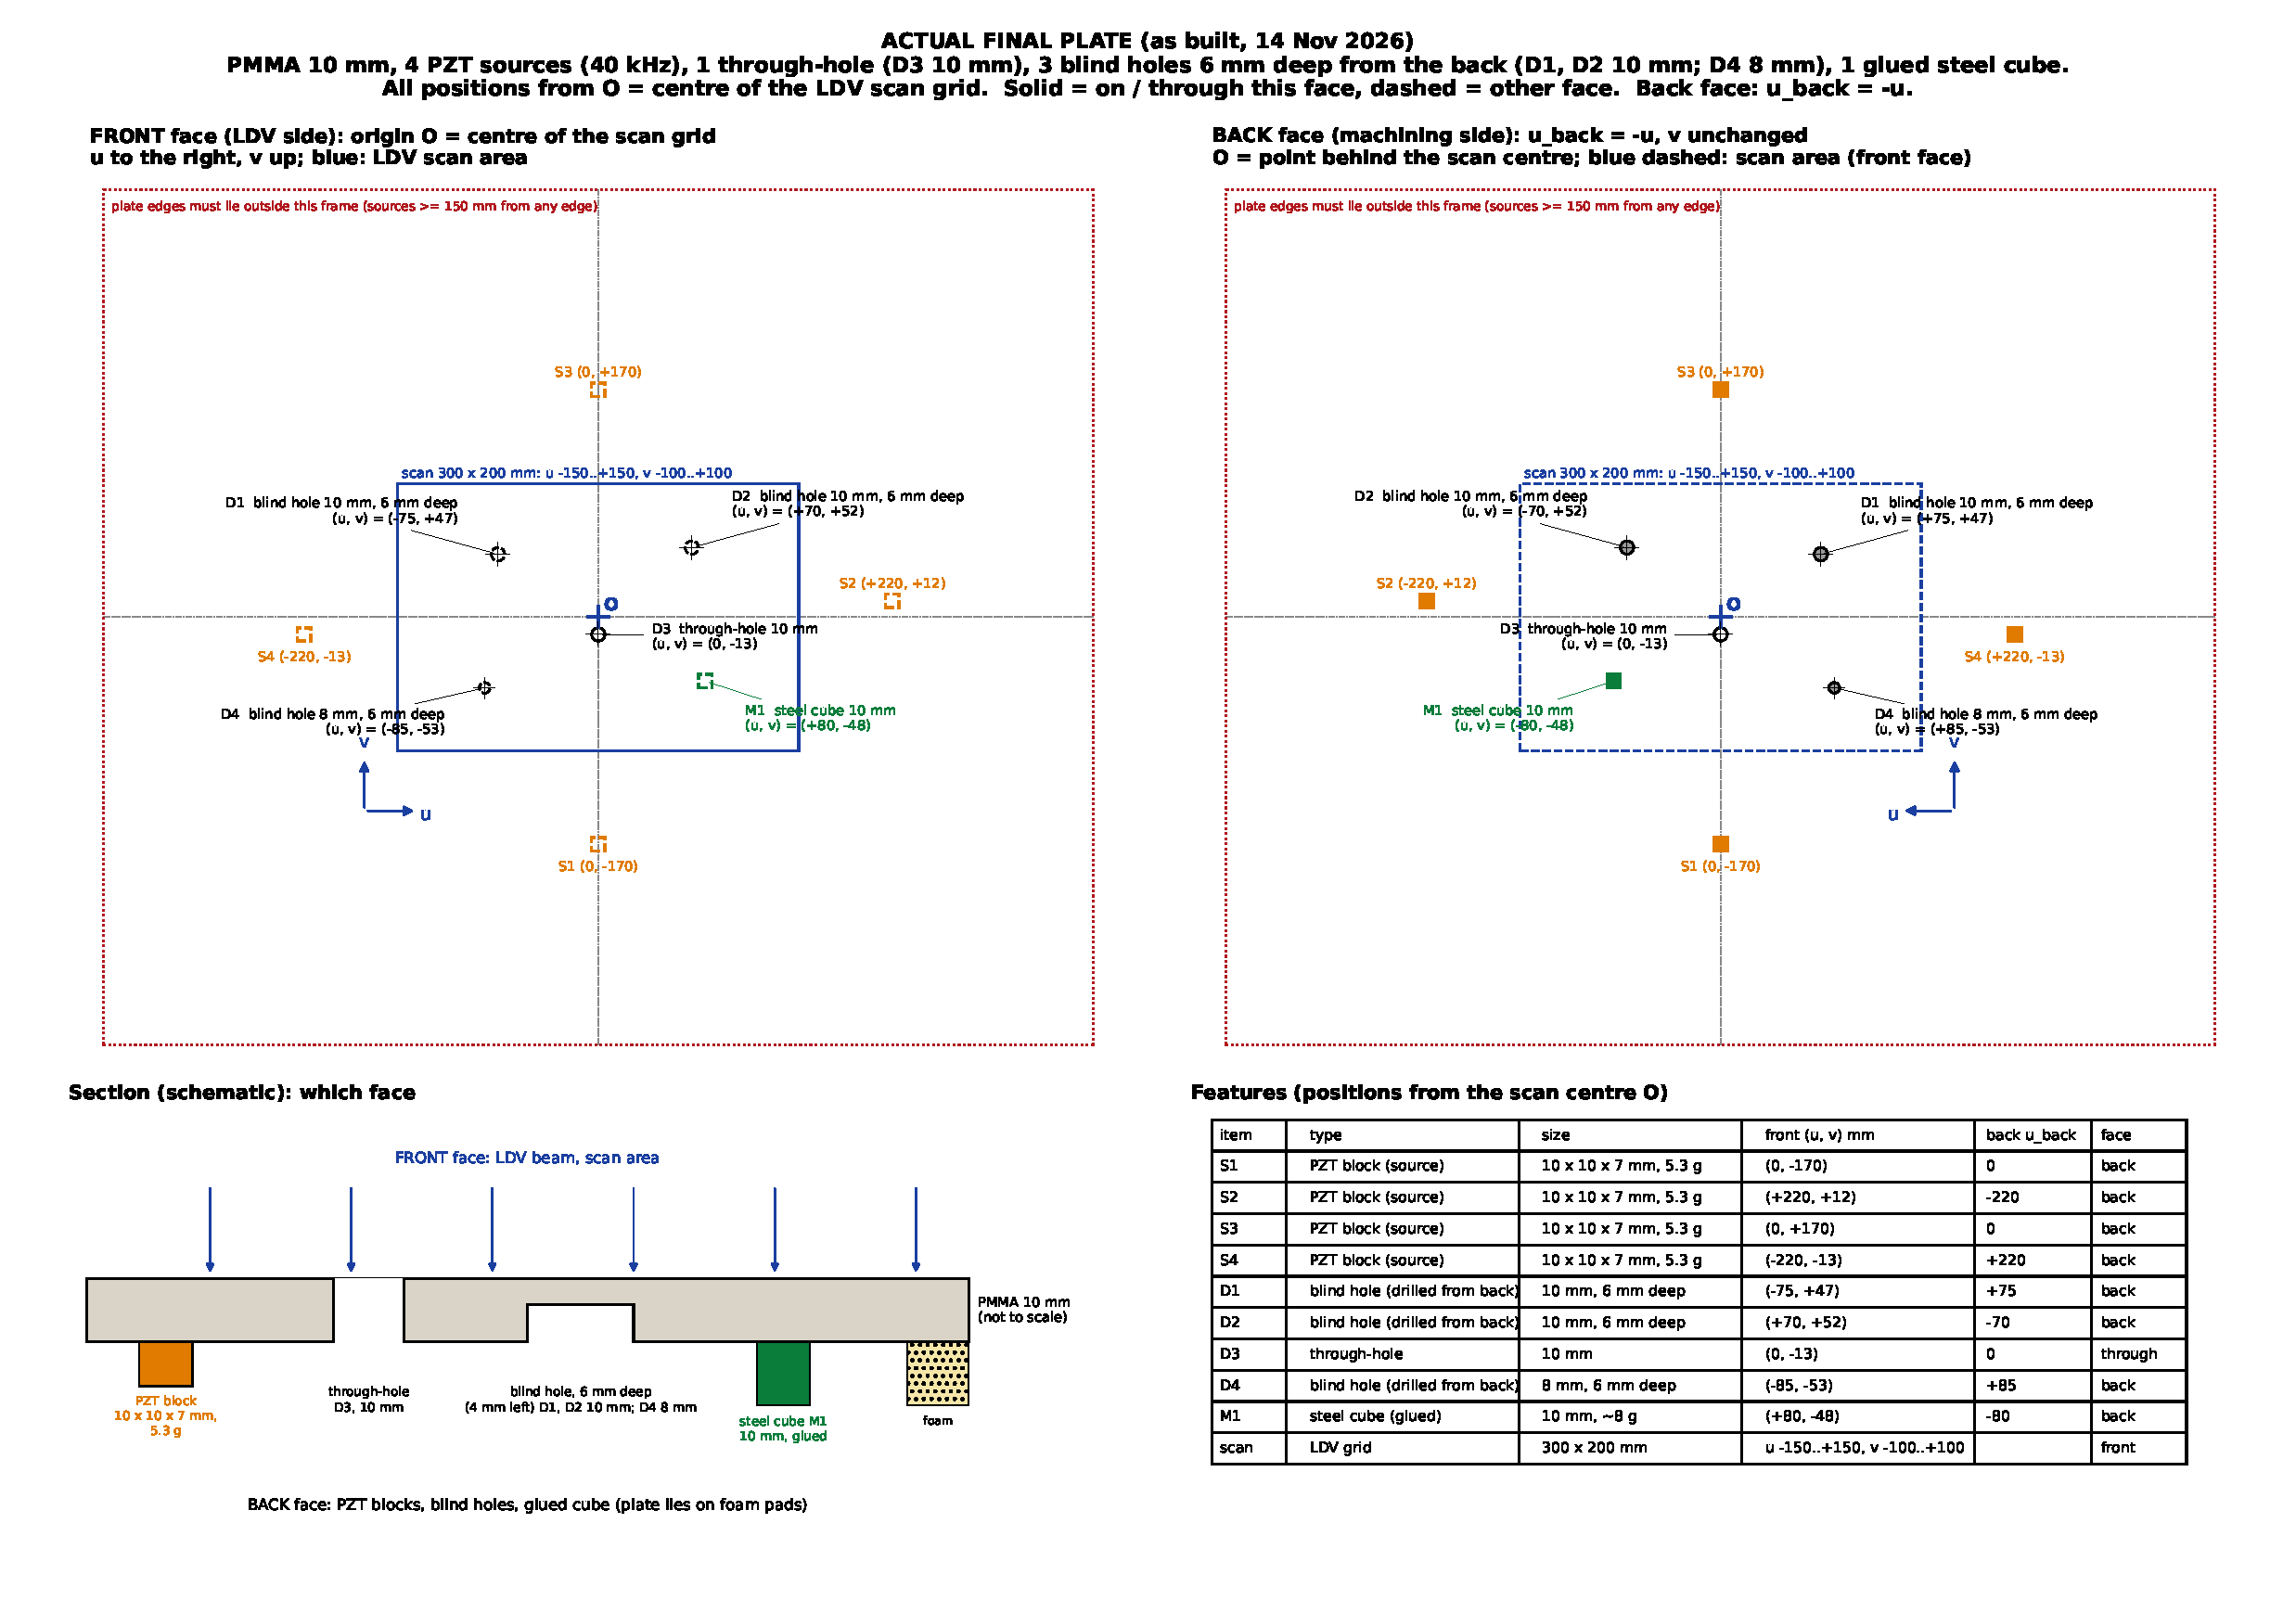
\includegraphics[width=\linewidth]{A1_specimen_full.pdf}
\caption{\textbf{Specimen drawing} (as built): front and back faces, section and coordinate table. PZT blocks 10$\times$10$\times$7\,mm, 5.3\,g.}\label{fig:drawing}
\end{figure}

\begin{figure}[ht]\centering
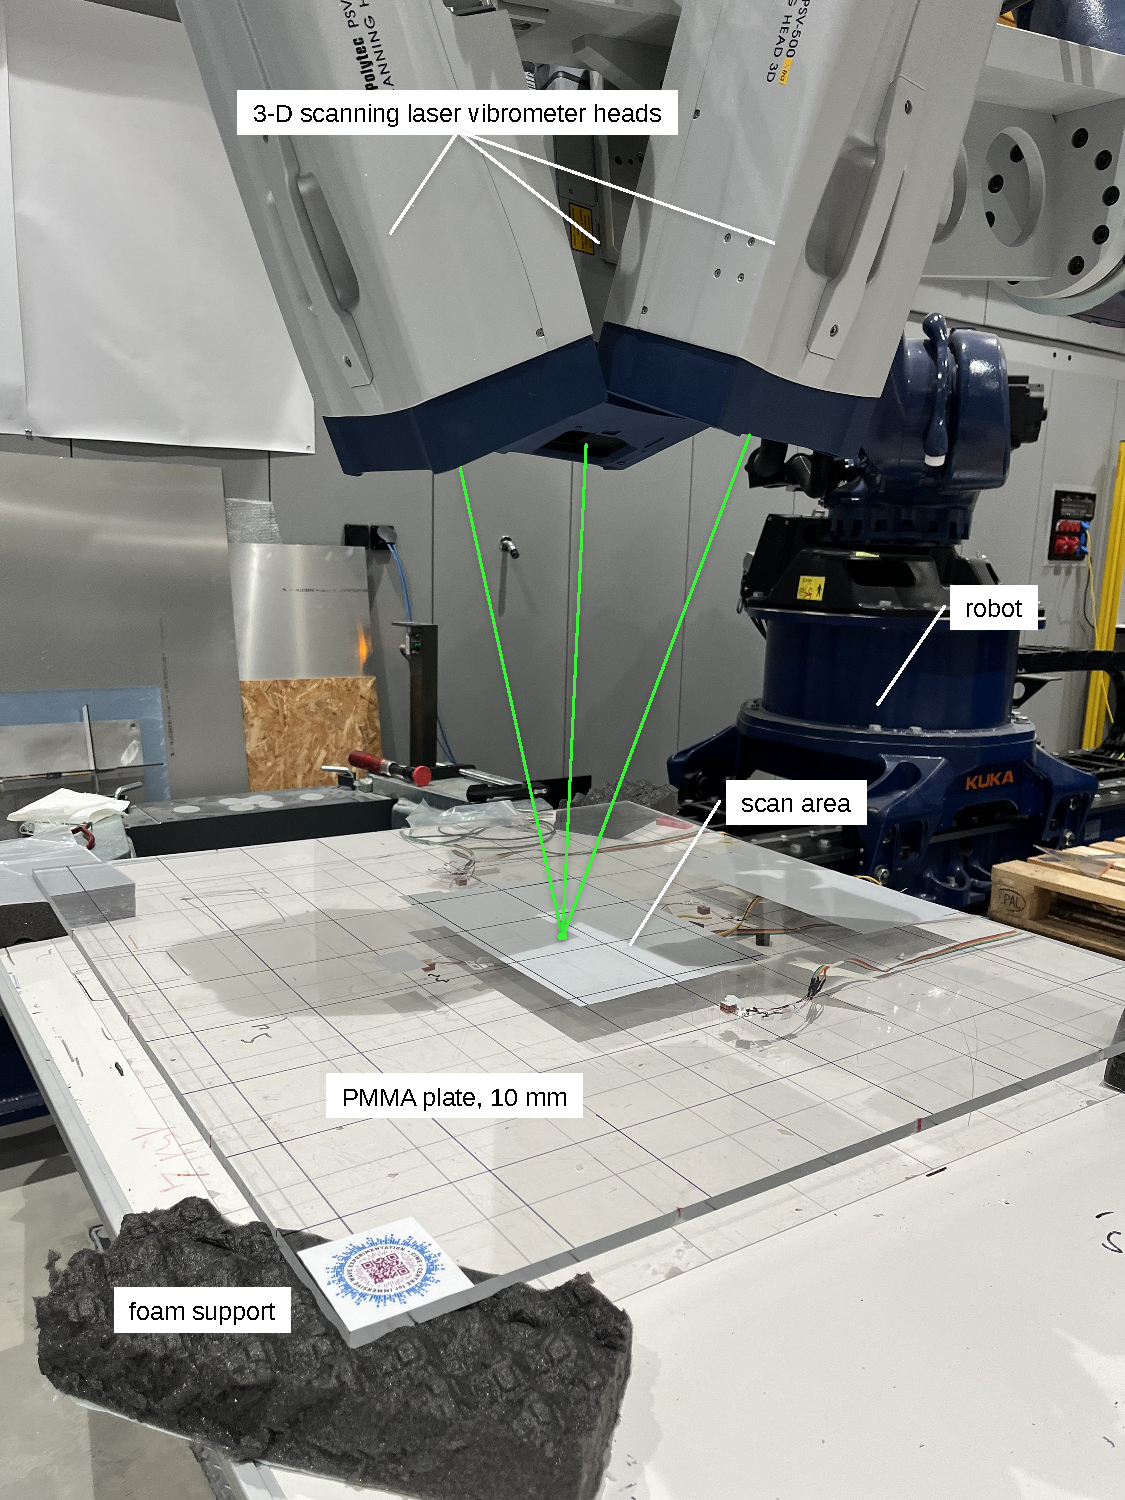
\includegraphics[width=0.5\linewidth]{A2_setup_edited.pdf}
\caption{\textbf{Laboratory setup}: 3-D scanning laser vibrometer on a robot above the PMMA plate (on foam supports); the white sheet marks the scan area; the three green beams converging on one scan point are drawn for illustration.}\label{fig:setup}
\end{figure}
